\chapter{Introduction}
\label{chp:b1}

Autonomous cars have received a great deal of attention over the last two
decades and started to be a reality in the last few years with several level of
autonomy from driving assistance level to full autonomy
\cite{Holstein2018EthicalAS}. In quest of fully autonomous vehicles, a number
of competitions were organized to stimulate researchers' interest
\cite{Buehler2007The2D, Buehler2009TheDU}. These events started with autonomous
cars driving on desert roads with only static obstacles and evolved to a point
where the cars survived a simple form of everyday traffic scenarios including
highway driving, overtaking, intersections, and parking. These challenges led
to state-of-the-art software architectures which decompose the driving problem
into components such as perception, planner, and controller. Each of these
components was also powered by state-of-the-art algorithms that shaped today's
autonomous vehicles.

Meanwhile, the progress in deep learning techniques along with the increase of
storage and computational power in the computer market made a breakthrough in
computer vision. These advances not only boosted the decomposition-based
approaches in perception side, but also revived the existing idea of learning a
mapping from raw camera images to steering commands \cite{Bojarski2016EndTE},
which is followed by the idea of learning driving affordance indicators such as
distance to the center of the ego lane, orientation of the car relative to the
road, and distance to the other cars so that steering and speed commands can be
computed with a dedicated controller based on these affordances
\cite{Chen2015DeepDrivingLA}.

Being an elegant and promising solution, learning affordances from raw
images requires additional tooling for data acqusition in order to compute and
record affordance indicators per image. The choice of affordance indicators for
a smooth driving experience also presents its own challenges.

Learning a direct mapping to the steering commands quickly reaches its limit
when the driving scenario becomes more complicated than tracking a curvy
road. Introduction of traffic regulations, overtaking, and lane keeping
policies remain too abstract to be captured in such a mapping. Furthermore,
human drivers tend to take different actions at different times even for the
same scenarios. Different actions on similar raw images in the training set
easily confuses the model \cite{Chen2015DeepDrivingLA}. Last but not least,
end-to-end nature of this approach presents difficulties in understanding and
debugging the behavior of the vehicle.

Existing decomposition-based approaches heavily depend on a high-definition map
of the driving environment, which often loses its validity due to changing
streets or constructions on the roads. Autonomous driving in urban scenarios
without an accurate map has been studied extending an existing traffic scene
segmentation dataset with ego lane, parallel lane, and opposite lane
annotations \cite{Meyer2018DeepSL}, but it is yet to be deployed and tested on
a car. For novel methods like this instance, a low-cost and risk-free solution
for initial on-road testing could be the use of a small-scale car.

Present small-scale driverless car studies either focus on directly learning
steering commands from the images \cite{Bechtel2017DeepPicarAL,
Do2018RealTimeSC} or implement a decomposed architecture using traditional
computer vision techniques to detect ego lane lines and few traffic signs
\cite{Blaga2018MiniatureAV}. Despite the existence of powerful small-scale
autonomous car platforms in the hardware side \cite{Karaman2017ProjectbasedCA},
related studies in the software side fail to keep up with the advances in
self-driving car technologies. One possible reason behind this lag could be the
lack of datasets for mini cars.


\section{Problem Definition}

We seek autonomous driving solutions to a number of traffic scenarios specified
by a mini autonomous car competition, OpenZeka MARC 2019 \cite{OpenZekaMARC}.
Inspired by MIT racecar platform \cite{Karaman2017ProjectbasedCA}, OpenZeka
MARC is organized by OpenZeka and was held in Februrary 2018, May 2018, and
April 2019 with increasingly complex rules. The competition offers leagues for
high schools, universities, and other hobbyists including companies. Total of
13 teams took part in the competition in 2019. Being one of the teams which
completed the race in time, we won the third place in the university league out
of 7 teams.

Our requirements are mostly derived from the competition rules as follows:

\begin{itemize}
  \item The mini car shall follow lanes at up to 0.9 m/s speed in a two-lane
    road as depicted in Figure \ref{figure:openzeka-race-course}.
  \item The mini car shall detect traffic light and signs shown in Figure
    \ref{figure:openzeka-traffic-signs}.
  \item The mini car shall overtake a waiting car on the right lane and steer
    back to the right lane.
  \item The mini car shall reactively avoid obstacles.
  \item The car shall climb up and climb down the cloverleaf interchange given
    in Figure \ref{figure:openzeka-race-course}.
  \item The mini car shall choose to go straight when it encounters straight or
    right turn sign.
  \item The mini car shall stop on red light and move on green light.
  \item The mini car shall change to the left lane when it is close to a
    construction zone on the right lane as indicated by keep-left signs.
  \item The mini car shall be capable of passing a rough road section indicated
    by a loose gravel sign.
  \item The mini car shall wait for pedestrians on crosswalks indicated by
    pedestrian crossing signs.
  \item The mini car shall turn right after parking sign into the parking lot
    given in Figure \ref{figure:openzeka-race-course}.
  \item The mini car shall stop on any of the free parking slots.
\end{itemize}

\begin{figure}[h]
  \centering
  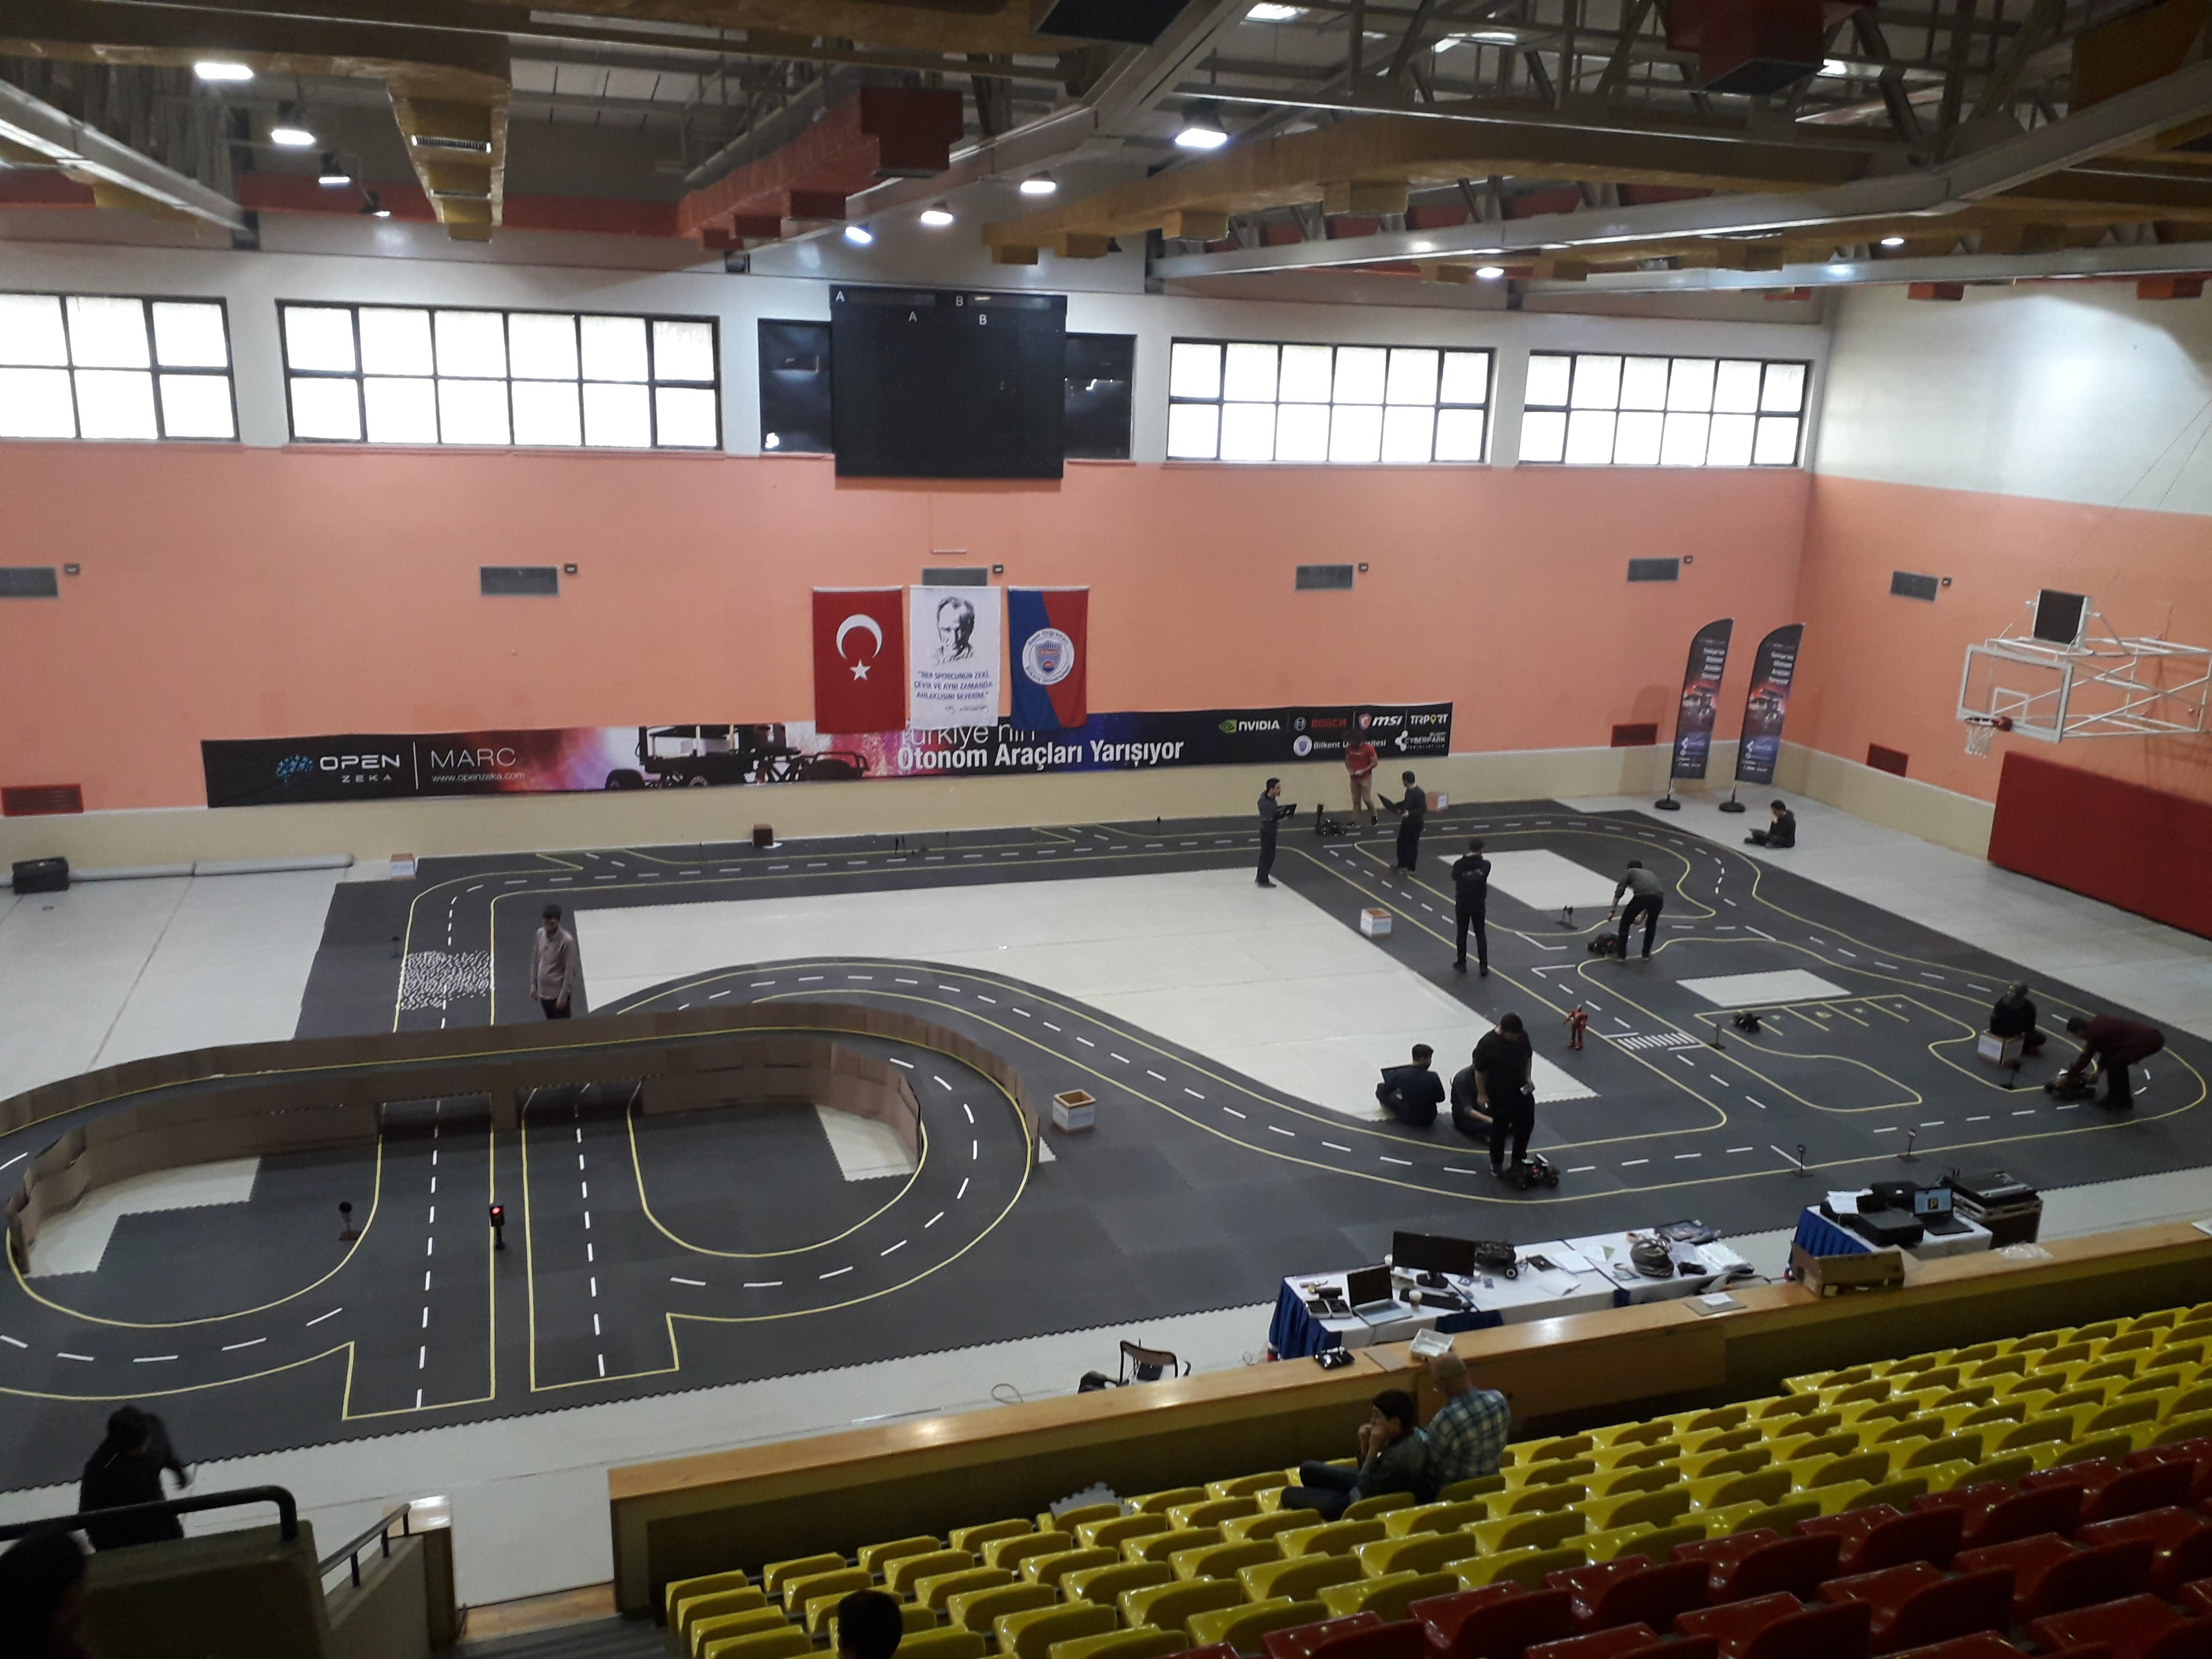
\includegraphics[width=.8\textwidth]{figures/openzeka-race-course.jpeg}
  \caption[OpenZeka 2019 MARC race course]{OpenZeka 2019 MARC race course.}
  \label{figure:openzeka-race-course}
\end{figure}

\begin{figure}[h]
  \centering
  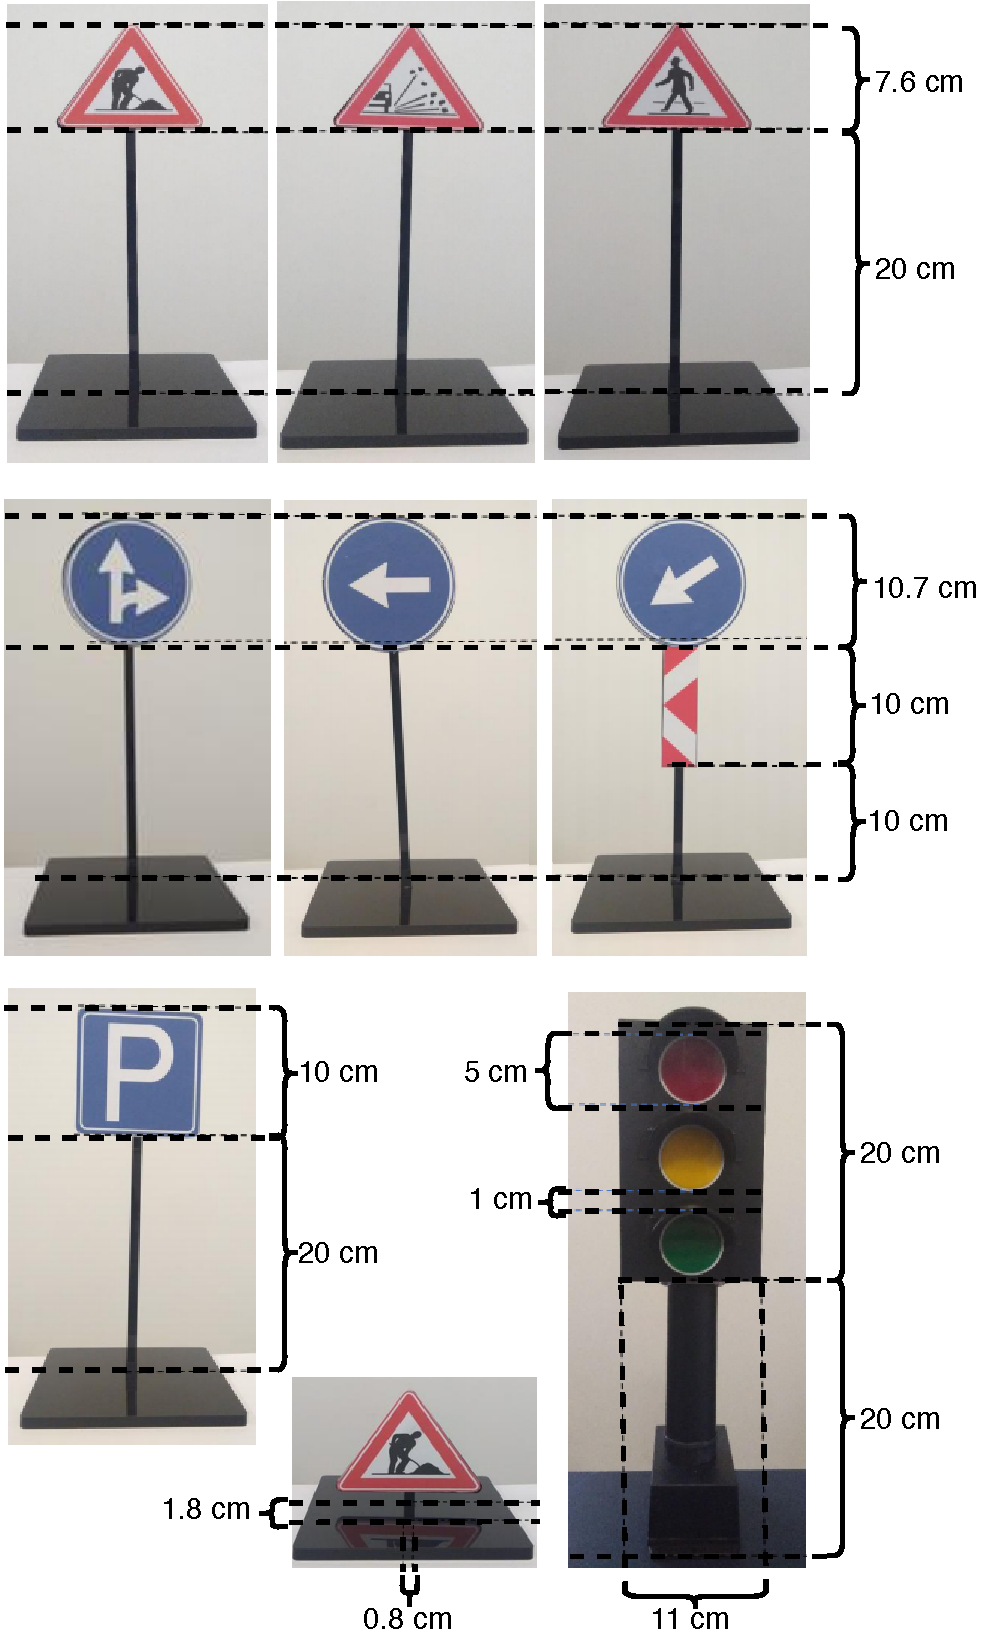
\includegraphics[width=.8\textwidth]{figures/openzeka-traffic-signs.pdf}
  \caption[Traffic signs and lights for mini cars]{Traffic signs and light
  specifically designed for mini cars by OpenZeka.}
  \label{figure:openzeka-traffic-signs}
\end{figure}

\section{Contributions}

The main contribution of our study is as follows:

\begin{itemize}
  \item \textbf{Pixel classification dataset for mini cars:} Existing traffic
    scene datasets are exclusively for real-scale cars \cite{Huang2018TheAD,
    Cordts2016TheCD, Geiger2012AreWR, Neuhold2017TheMV}. This poses a
    difficulty for on-road testing of the novel methods on mini-cars. We
    present a dataset with pixel-level annotations for mini cars.
  \item \textbf{Extended traffic sign and signal classification dataset:} We
    merge existing traffic sign classification datasets
    \cite{Timofte2009MultiviewTS, Stallkamp2012ManVC, Shakhuro2016RussianTS,
    Serna2018ClassificationOT, MaldonadoBascn2007RoadSignDA} for our scenarios
    and semi-automatically extend the dataset by cropping the segmented sign
    regions from our camera images.
  \item \textbf{Development of a novel lane detector:} We build our lane
    detector on the approach proposed by Meyer et al. \cite{Meyer2018DeepSL}.
    This approach essentially segments the road into ego lane, parallel lane,
    and opposite lane. It then extracts a center line for the ego lane. For our
    scenarios, we skip the opposite lane and further segment the parallel lane
    into right and left lanes. Unlike Meyer et al. \cite{Meyer2018DeepSL}, we
    are interested in finding center line curves for neighboring parallel lanes
    along with the ego lane. Our apprach saves us from analyzing the parallel
    lane pixels for right or left categorization.
  \item \textbf{Local optimal trajectory planner for structured environments:}
    It is common that state-of-the-art autonomous vehicles rely on detailed
    maps to provide a reference line to their local planner for structural
    environments (i.e., environments with explicit drivable corridors), often
    by means of a global planner \cite{Thrun2006StanleyTR,
    Montemerlo2009JuniorTS, Kato2018AutowareOB}. We implemented a Frenet
    optimal trajectory planner \cite{Werling2010OptimalTG} without a map using
    exclusively the online computed lane centers as a source of the reference
    line.
  \item \textbf{Decomposed architecture for autonomous driving:} Autonomous
    vehicle architectures span a wide range of computer science research areas
    including but not limited to computer vision, path planning, automata
    theory, control theory, and distributed systems. Each of these areas comes
    with many problems and various alternative solutions to those problems. We
    put together a decomposed architecture with a selected set of solutions
    from different domains.
\end{itemize}

\section{Organization}

The organization of this thesis as follows:

Chapter 2 discusses various autonomous driving approaches and algorithms used
in search of autonomy highlighting their advantages and disadvantages.

Chapter 3 presents our hardware configuration and software architecture at a
high level. In Chapter 3, we also introduce our simulation environment that
accelerated the development and verification processes.

Chapter 4 provides a detailed description of our scene interpretation module in
which we implement perception and behavior planning capabilities of the car.
First, we present our segmentation model which is used to parse the current
scene into lanes and traffic signs. Second, we introduce our lane center line
extraction method based on the parsed lane semantics. Third, we discuss our
traffic sign classification approach on the sign regions proposed by
segmentation model. Next, we review our obstacle detection method. Finally,
we explain our behavioral layer that implements a hierarchical finite state
machine that regulates the decisions made by the car based on the perception
capabilities.

Chapter 5 is dedicated to our trajectory planner and control algorithms. We
start with introducing Frenet frame on a lane segment and then we explain how
we plan an optimal trajectory based on the lane center lines provided by the
scene interpretation module. In the second half of this chapter, we derive and
tune pure pursuit control algorithm that computes steering commands to execute
our optimal trajectories.

Chapter 6 presents our datasets, experiments, and results. In Chapter 6, we
evaluate our segmentation and classification models. Then, we demonstrate the
actions performed by our car in response to various traffic scenarios and
compare them with the actions taken by a human driver.

Chapter 7 concludes our arguments by summarizing our approach to autonomous
driving, highlighting its limitations and suggesting directions for future
work.
